\documentclass{beamer}
\usepackage{graphicx}
\usepackage{animate}
\usepackage{caption}
\usepackage{subcaption} % For subfigures
\captionsetup{font=footnotesize}

\usetheme{Madrid}
\usecolortheme{default}

\begin{document}

\title[]{Training augmented interpolation}

\author[FONSECA HINCAPIE Diana Sol Angel]{FONSECA HINCAPIE Diana Sol Angel}
\date[23 August 2023]{23 August 2023}

\definecolor{uoftblue}{RGB}{6,41,88}
\setbeamercolor{titlelike}{bg=uoftblue}
\setbeamerfont{title}{series=\bfseries}
\begin{frame}
\titlepage
\begin{center}

\includegraphics[width=0.2\textwidth]{images/inria.png}

\includegraphics[width=0.2\textwidth]{images/logo_irma.png}

\includegraphics[width=0.2\textwidth]{images/logo_unistra.jpg}

\end{center}
\end{frame}

\section{Objectives}
\begin{frame}{Objectives}
  The main objective of this project is to solve simple transport equations using the Semi-Lagrangian scheme and the deep interpolation operator.
  
  \vspace{0.5cm}

  For this the specific objectives are: \\

  \vspace{0.3cm}

  \begin{itemize}
    \item Implement the PINNs strategy. 
    \item Implement the Semi-Lagrangian scheme.
    \item Study of the error. 
  \end{itemize}

\end{frame}



\section{Introduction}
\begin{frame}{Introduction}
    
    We are interested in the resolution of transport equations, the aim is to find a way to increase the accuracy of the method using deep learning
    
    \vspace{0.3cm}

    \textbf{Advection Equation}
 
    \begin{equation}
        \begin{cases}
        \frac{\partial u}{\partial t} + a \frac{\partial u}{\partial x} = 0 \quad (x,t) \in \Omega \times (0,T) \\
         u(x,t=0) = u_0(x) \quad x \in \delta \Omega \\
        \end{cases}
    \end{equation}
    \\

    Has an analytical solution equal to: 
    $$
    u(t, x)=u_0(x, x-at)
    $$
    
\end{frame}

\section{Context of the project}
\begin{frame}{General context}
    %Pourquoi on fait ce projet pourquoi c'est important
    This internship was supervised by the National Institute for  Research in Digital Science and Technology (INRIA)and the University team \textbf{Modeling and Control} of the IRMA laboratory. 
    \begin{figure}
        \centering
        
\includegraphics[width=0.3\textwidth]{images/inria.png}
        
\includegraphics[width=0.3\textwidth]{images/logo_irma.png}
    \end{figure}

\end{frame}

\section{Theorical framework}
\subsection{Semi Lagrangian Scheme}
% \begin{frame}{Semi-Lagrangian Scheme}
    
    \begin{figure}
        \centering
        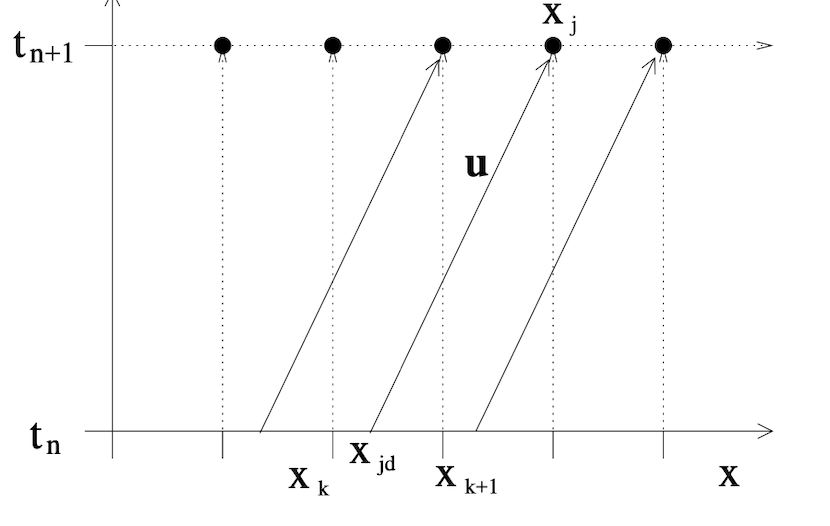
\includegraphics[width=0.8\textwidth]{images/11.png}
        \caption{Semi-Lagrangian in 1D}
    \end{figure}

\end{frame}
\begin{frame}{Semi-Lagrangian Scheme}
    
    \begin{figure}
        \centering
        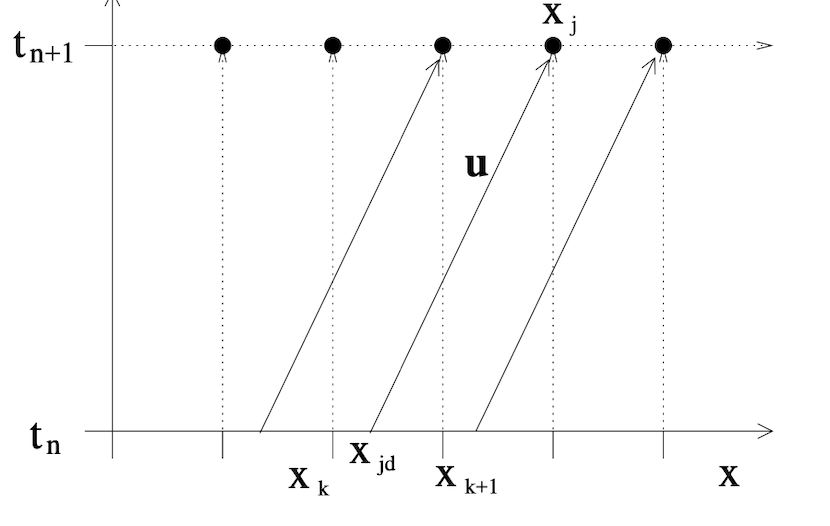
\includegraphics[width=0.8\textwidth]{images/11.png}
        \caption{Semi-Lagrangian in 1D}
    \end{figure}

\end{frame}
\subsection{Lagrange Interpolation Operators}
\begin{frame}{Lagrange Interpolation Operators}
    \textbf{The Lagrange interpolation operator:}
    \begin{equation*}
        \mathcal{I}_h^m(f)(x)=\sum_{i=1}^m f\left(x_i\right) P_i(x)
    \end{equation*} 
    with $P_i\left(x_j\right)=\delta_{i j}$


    \textbf{The Deep Lagrange Interpolation:}
    \begin{equation*}
        \mathcal{I}_d^m(f)=\sum_{i=1}^n \frac{f\left(x_i\right)}{u_\theta\left(x_i\right)} P_i(x) u_\theta(x)=\mathcal{I}^m\left(\frac{f}{u_\theta}\right) u_\theta(x)
    \end{equation*}

    With $P_i\left(x_j\right)=\delta_{i j}$
    Using this choice, we obtain that $\mathcal{I}_d(f)\left(x_i\right)=f\left(x_i\right)$ as the classical interpolator.
    

    % \textbf{ $u_{\theta i}$ Function:}

    % \begin{equation*}
    %     u_{\theta_i}(x)= u_0(x + \epsilon -at)

    % \end{equation*}
\end{frame}

\subsection{$u_{\theta i}$ Function}
\begin{frame}{$u_{\theta}$ Function:}

    \textbf{How do we choose $u_{\theta}$ ?}
    
    We use a neural network which will approximate the $u_\theta(x)$ function. 
    $$
    u_{pred} = u_{\theta}(x ,t, \mu, \sigma, a)
    $$

    We train a neural network with a \textbf{Physics Informed Neural Network} strategy, and we use the previous interpolation to approximate
    the solution of the PDE.

\end{frame}


\begin{frame}{Universal Approximation Theorem}
    
    Any continuous function  $f : [0, 1]^{n} \rightarrow [0, 1]$  can be approximated arbitrarily well by a neural network with at least 1 hidden layer with a finite number of weights.

    Even if neural networks can express very complex functions compactly, determining the precise parameters (weights and biases) required to solve a specific PDE can be difficult.
    
\end{frame}
\subsection{Physics informed neural network}
\begin{frame}{Physics informed neural network}
    \begin{itemize}
        \item PINNs are a type of universal function approximators that can embed the knowledge of any physical laws that govern a given data-set in the learning process, and can be described by PDEs.
        \item They approximate PDE solutions by training a neural network to minimize a loss function; it includes terms reflecting the initial and boundary conditions along the space-time domain’s boundary and PDE residual and data points.
        \item PINNs training can be thought of as a supervised and/or supervised learning approach.
    \end{itemize}

\end{frame}
\begin{frame}{Physics Informed Neural Network}
    
    \begin{figure}
        \centering
        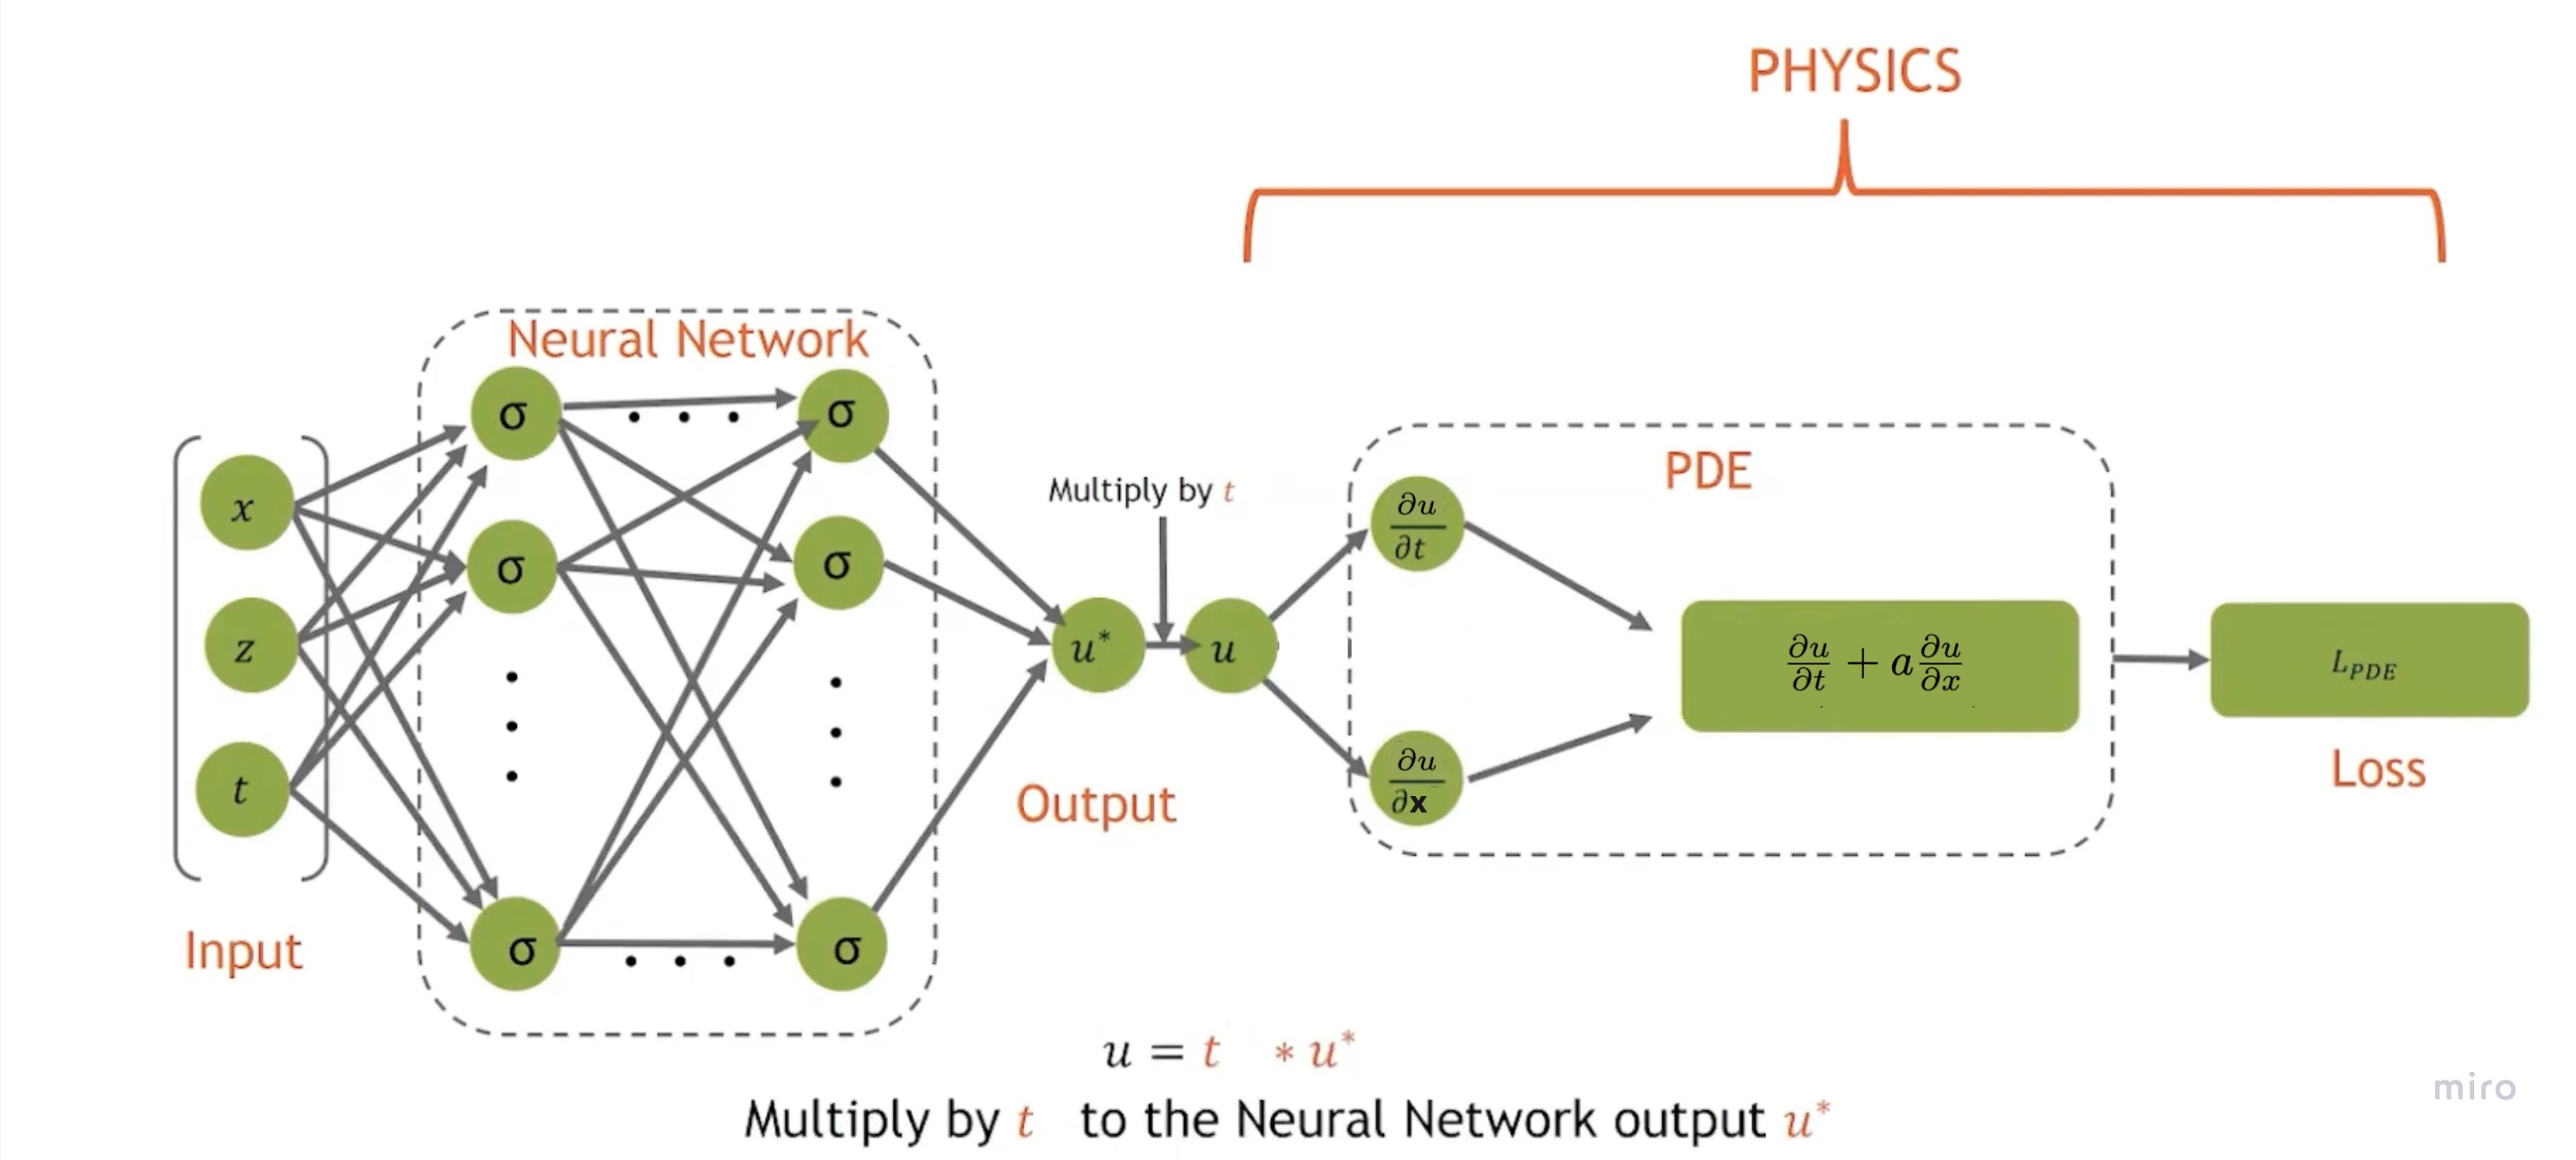
\includegraphics[width=0.9\textwidth]{images/loss.jpg}
        \caption{PINN strategy - Source: Youtube video "Introduction to PINNs"}
    \end{figure}

\end{frame}
\begin{frame}{Methodology}
    We have an initial conditions $u_0$:  
    \begin{align*}
        u_0 &= \exp\left(-\frac{(x - \mu)^2}{\sigma}\right)
    \end{align*}
    \\
    with $\mu$ the mean and $\sigma$ the variance of the Gaussian distribution.
    
    \vspace{0.3cm}

    Using the \textbf{PINNs} approach we determine the parameters $\beta$ of the NN, $u_\theta$:
    $$
    u_{pred}(x,t,\beta) = u_0(x) + b_c(x) u_\beta^{NN}(x,t)
    $$
    We assume then that:
    $${u_{pred}}(x,t,\beta)\approx u(x,t)$$ 

    Where the \textbf{Loss function} is defined as:
    $$
    L(\beta) = L_{data}(\beta) + L_{physics}(\beta) + L_{SBC}(\beta) + L_{TBC}(\beta)+ L_{IC}(\beta)
    $$


\end{frame}

\begin{frame}{Implementation}
   
     
\end{frame}


\subsection{Results}
\begin{frame}{Results PINNs startegy}

    \textbf{{Finding $u_\theta$ using PINNs}}
    For training the neural network and solving the transport equation we used the following parameters:
    \vspace{0.3cm}
    \begin{itemize}
        \item[--] $min = 0.$
        \item[--] $xmax = 1.$
        \item[--] $tmin = 0.$
        \item[--] $tmax = tf$
        \item[--] $a = 1.$
        \item[--] $learning$ $rate = 1e-3$
        \item[--] $min$ $mean = 0.45$
        \item[--] $max$ $mean = 0.55$
        \item[--] $min$ $variance = 0.01$
        \item[--] $max$ $variance = 0.05$
    \end{itemize}
   
\end{frame}


\begin{frame}{Unsupervised learning}
    We trained our NN with 40.000 epochs and 50.000 collocation points, the best loss we obtained was: 3.76e-04 With a Gaussian initial condition with mean $\mu= 0.49$ and variance $\sigma= 0.04$
    \begin{figure}
        \centering
        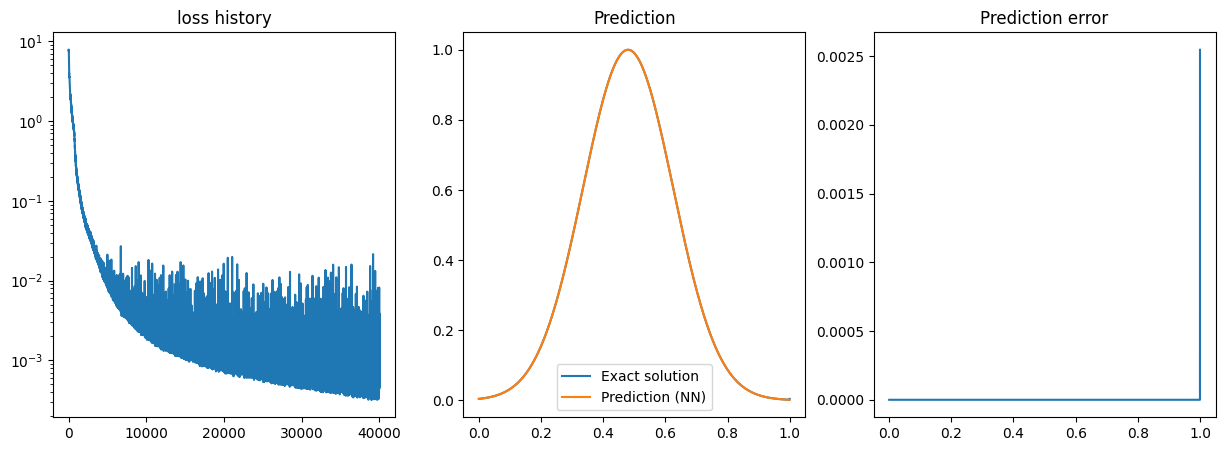
\includegraphics[width=0.3\textwidth]{images/nsup1.png}
        \caption{t=0}
        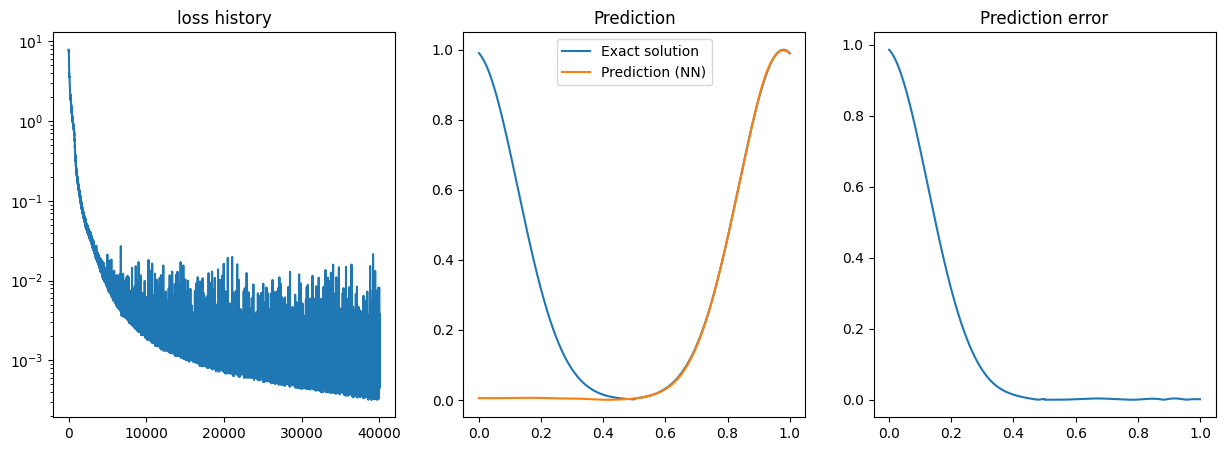
\includegraphics[width=0.3\textwidth]{images/nsup3.png}
        \caption{t=0.5}
        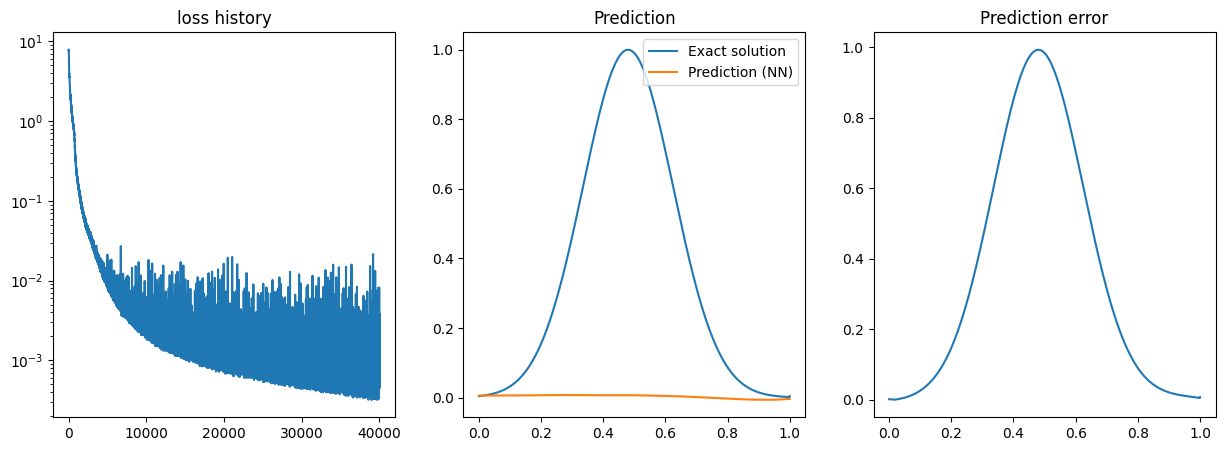
\includegraphics[width=0.3\textwidth]{images/nsup5.png}
        \caption{t=1.}
    \end{figure}

\end{frame}

 
\begin{frame}{Supervised learning}
    We trained our NN with 40.000 epochs and 15.000 data points, the best loss we obtained was: 3.21e-04 With a Gaussian initial condition with mean $\mu= 0.48$ and variance $\sigma= 0.042$
    \begin{figure}
        \centering
        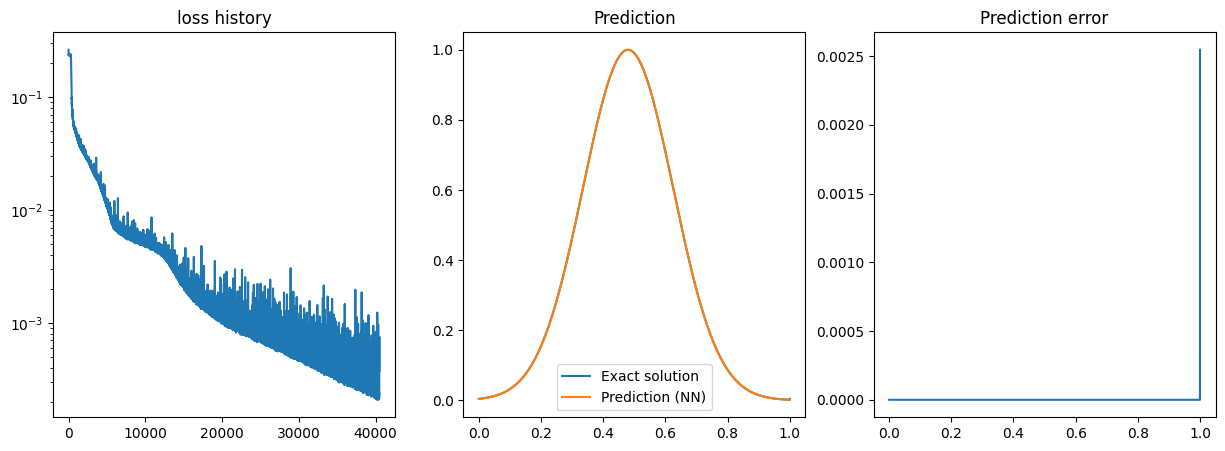
\includegraphics[width=0.3\textwidth]{images/data1.png}
        \caption{t=0}
        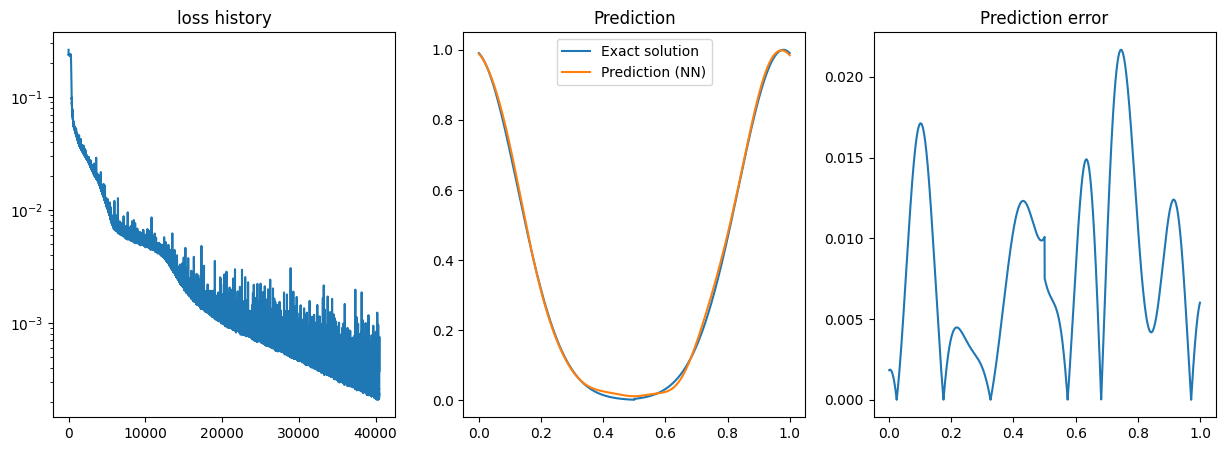
\includegraphics[width=0.3\textwidth]{images/data3.png}
        \caption{t=0.5}
        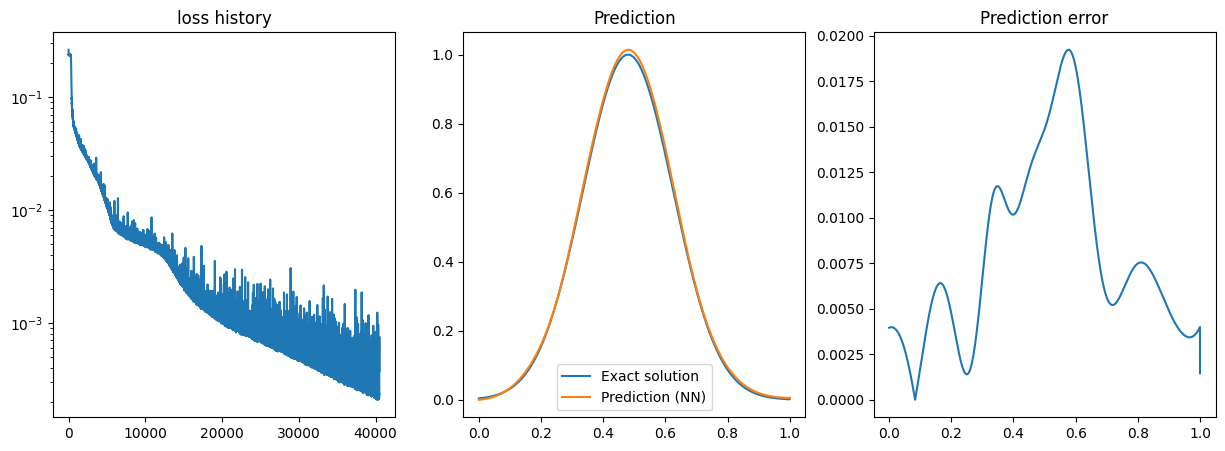
\includegraphics[width=0.3\textwidth]{images/data5.png}
        \caption{t=1.}
    \end{figure}
\end{frame}
\begin{frame}{Unsupervised and Supervised learning}
    We trained our NN with 40.000 epochs, 50.000 collocation points and 10.000 data points, the best loss we obtained was: 7.80e-04 With a Gaussian initial condition with mean $\mu= 0.5$ and variance $\sigma= 0.35$
    \begin{figure}
        \centering
        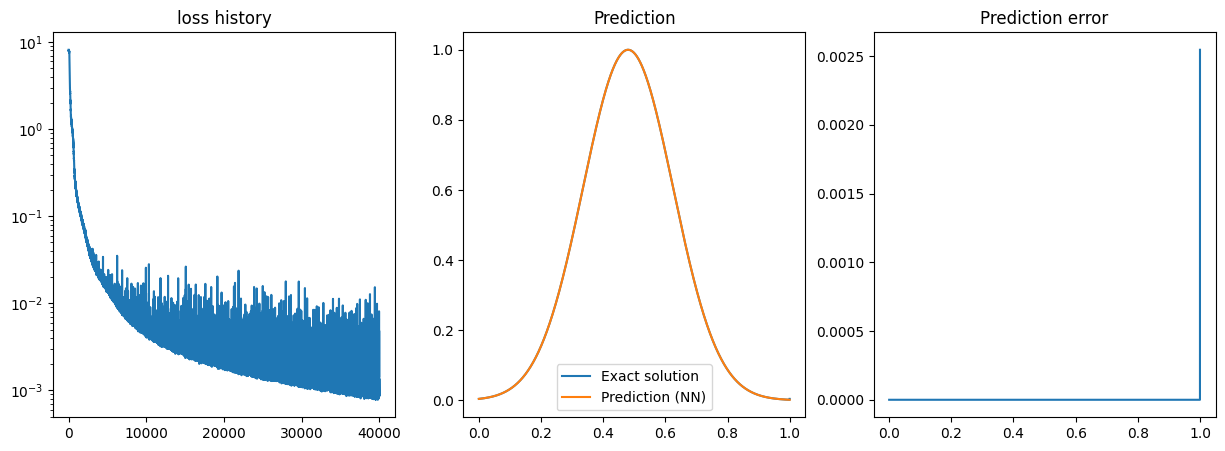
\includegraphics[width=0.3\textwidth]{images/r1.png}
        \caption{t=0}
        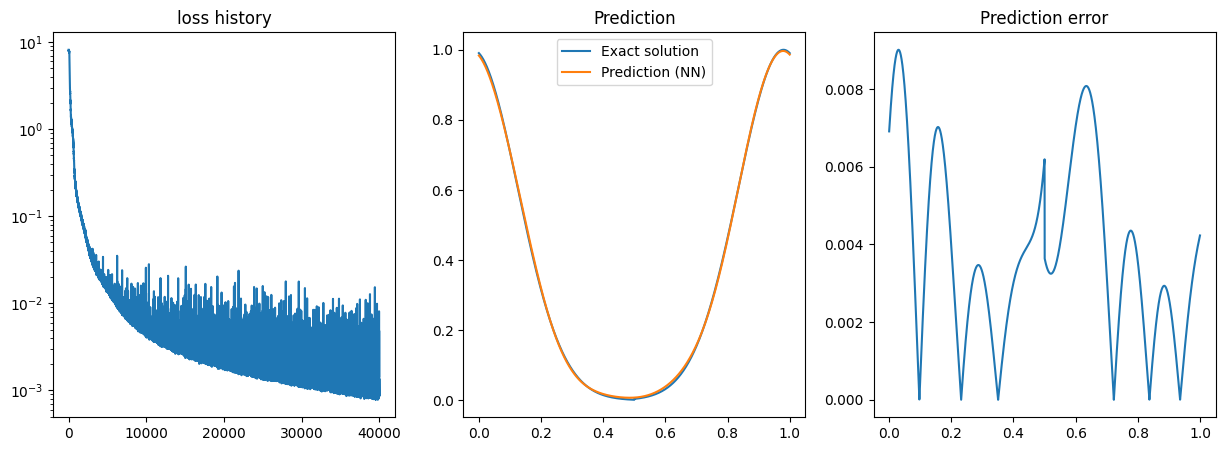
\includegraphics[width=0.3\textwidth]{images/r3.png}
        \caption{t=0.5}
        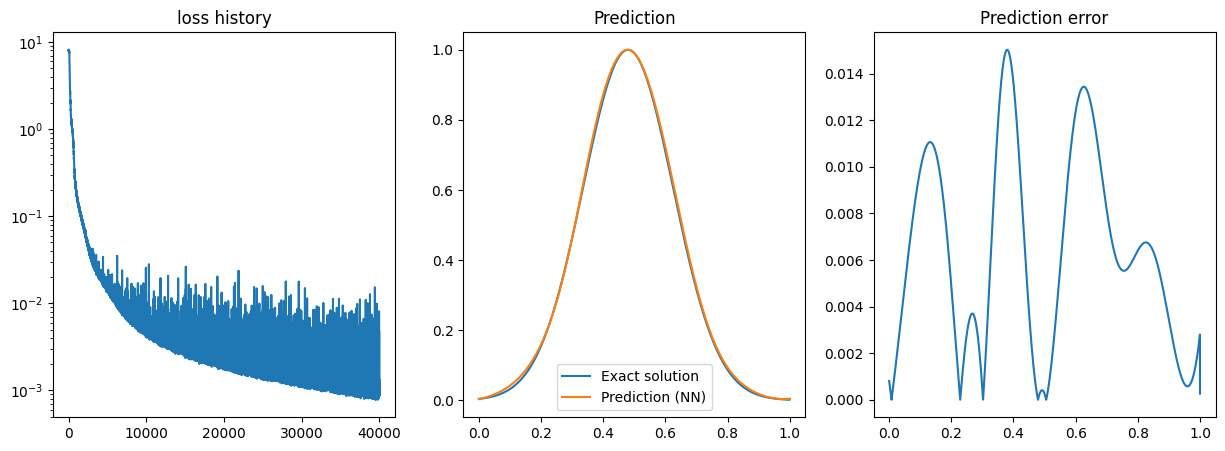
\includegraphics[width=0.3\textwidth]{images/r5.png}
        \caption{t=1.}
    \end{figure}
     
\end{frame}

\begin{frame}{Results}
    \textbf{Convergence Results}
 
    \textbf{In space} 
    \begin{figure}
       \centering
       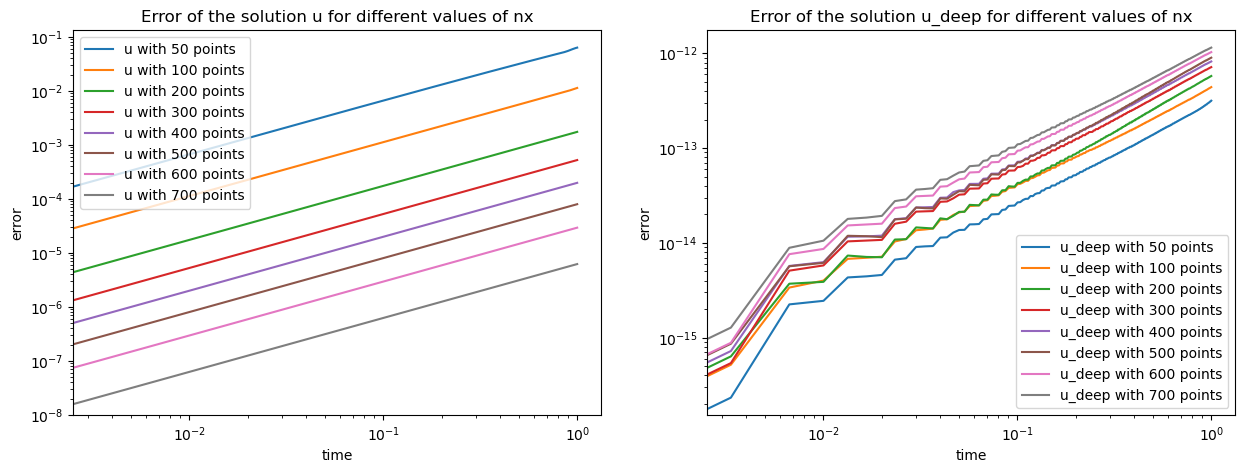
\includegraphics[width=0.5\textwidth]{images/conv1.png}
       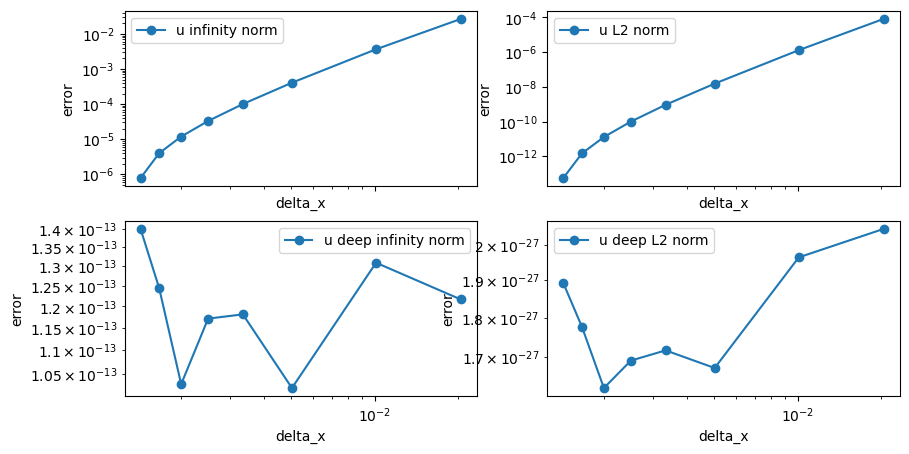
\includegraphics[width=0.5\textwidth]{images/conv2.png}
   \end{figure}
     
 \end{frame}
\begin{frame}{Average gain}
   
     
\end{frame}

\begin{frame}{Creneau }
   
     
\end{frame}


\subsection{Conclusion}
\begin{frame}{Conclusions}
    
    Our findings demonstrate that the Semi-Lagrangian scheme combined with deep learning approaches shows promise in improving the accuracy of transport equation solutions. 
    However, there is still further research to be done implementing the deep Lagrange interpolation with PINNs to optimize the deep learning models and explore their full 
    potential in solving complex transport equations.
    

\end{frame}
\begin{frame}{Final remarks}

    \textbf{Outlook:}\\


    \textbf{Personal feedback:}\\
  

\end{frame}

\section{Bibliography}
\begin{frame}{Bibliography}

    \begin{itemize}
        \item[1] Semi Lagrangian \url{https://www.youtube.com/watch?app=desktop&v=egnsVOvJYIA}
        \item[2] Neural Networks and the Universal Approximation Theorem Milind Sahay Published in
        Towards Data Science
        \item[3] Scientific  Machine  Learning  Through  Physics–Informed  Neural Networks: Where we are and What’s Next,
        S. Cuomo, V. Schiano Di Cola, F. Giampaolo,  G. Rozza,  M. Raissi, F. Piccialli1
    \end{itemize}
    
\end{frame}

\end{document}